\block{\begin{blockbody}\section{Applying GIANI to 3D analysis of mouse embryos}
    \tfont
    \setlength{\unitlength}{\textwidth}
    {\centering\def \bwidth {\unitlength}
\begin{tikzpicture}[every node/.style={inner sep=0}]
    \node (input) at (0.0, 0.0) {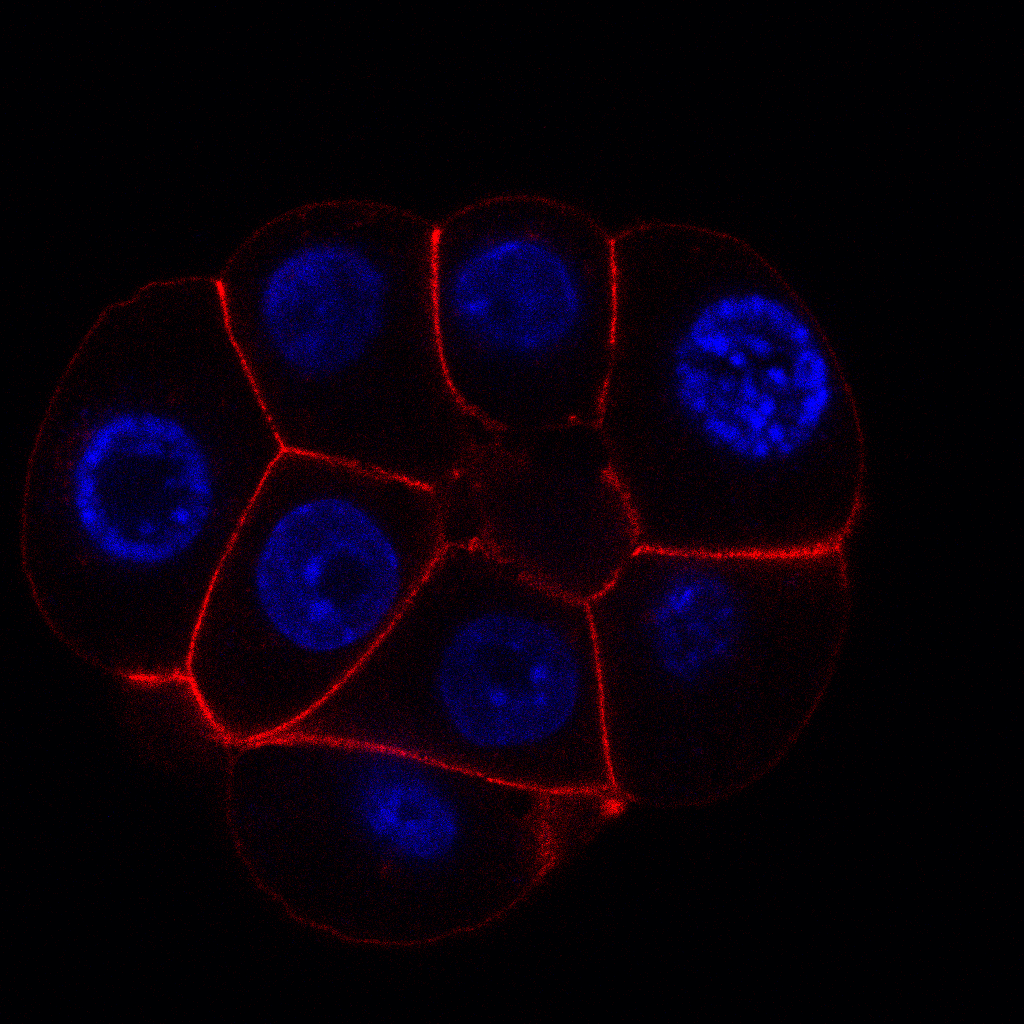
\includegraphics[width=0.3\unitlength]{images/ExampleSlice.png}};
    \node (nuc) at (0.33\unitlength, 0.0) {
\includegraphics[width=0.3\unitlength]{images/NucSeg.png}};
    \node (cells) at (0.66\unitlength, 0.0) {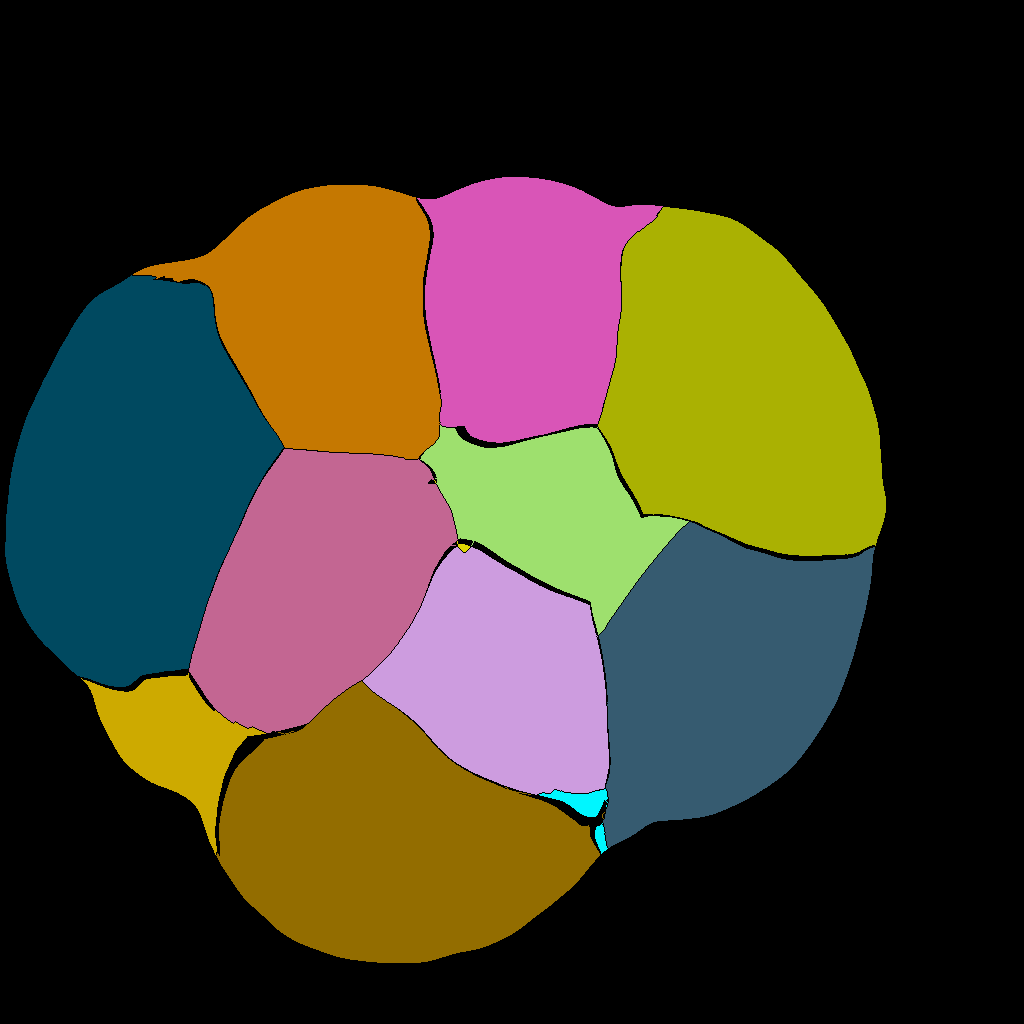
\includegraphics[width=0.3\unitlength]{images/CellSeg.png}};
    \path[arrow] (input) -- (nuc);
    \path[arrow] (nuc) -- (cells);
\end{tikzpicture}\par}\par
    \vs
    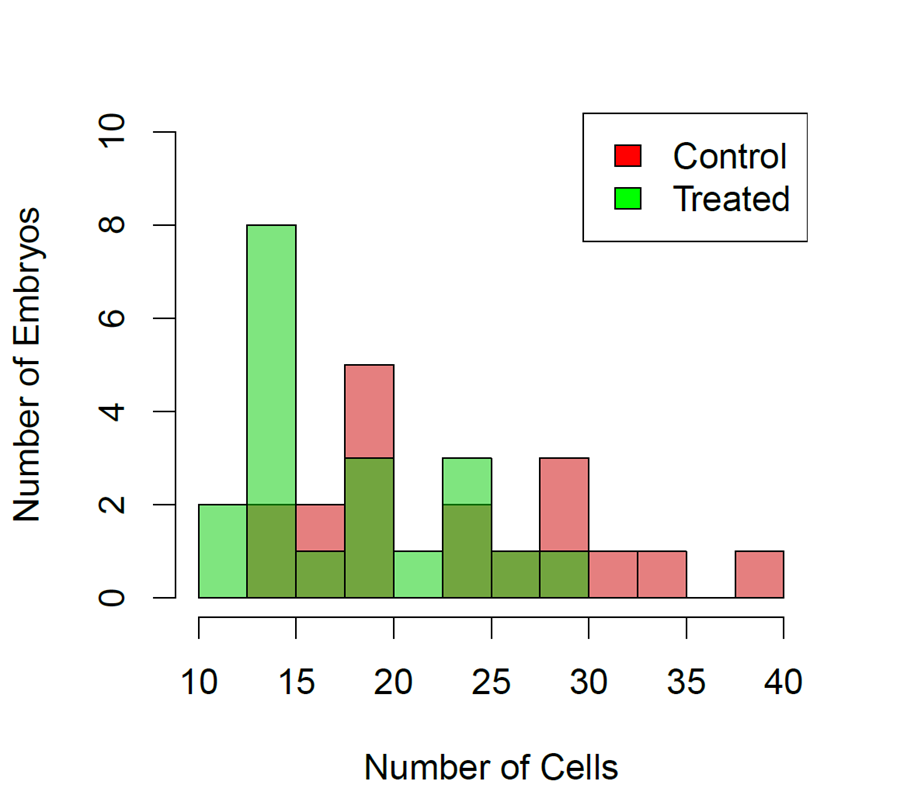
\includegraphics[width=0.48\textwidth]{images/CellCount.png}\hfill
    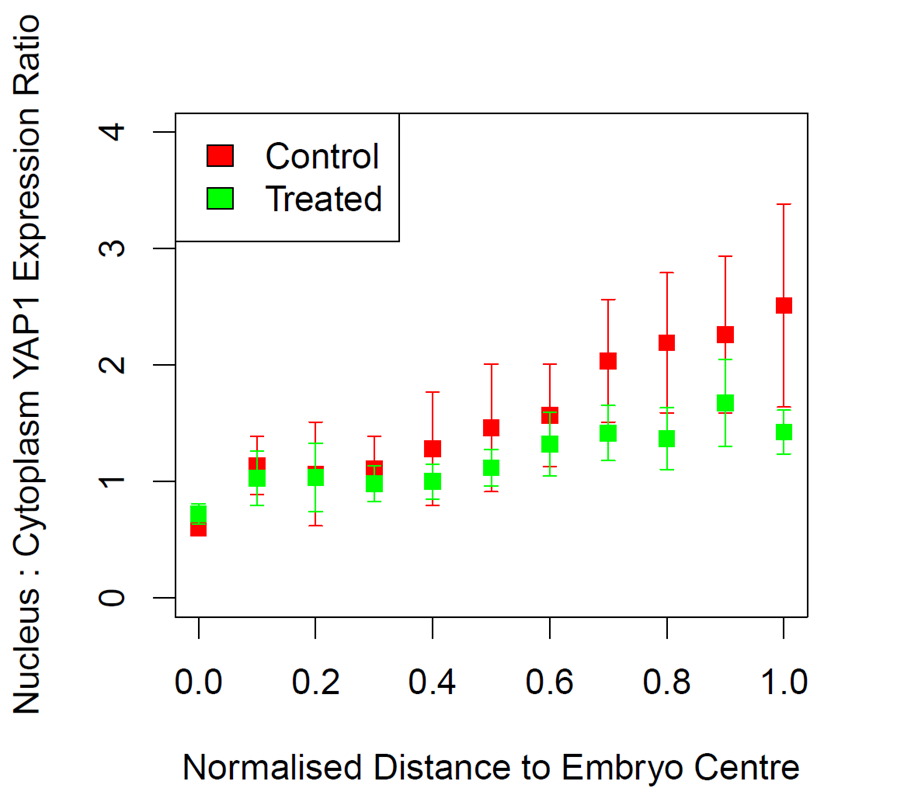
\includegraphics[width=0.48\textwidth]{images/YapExpress.png}\par
    \vs
    We used GIANI to analyse 3D image data of two populations of mouse embryos acquired by confocal microscopy - an example segmentation of one such dataset is shown above. Preliminary results indicate differences in the number of cells present in the two embryo populations (at the same stage of development) and differences in the expression profile of YAP1 within the embryos.
\end{blockbody}}